\newcommand{\hamburger}{%
  \vbox{%
    \hrule width 1em height 1pt\smallskip
    \hrule width 1em height 1pt\smallskip
    \hrule width 1em height 1pt}%
}
\chapter{MRIM Operations}
\gls{rsrm} simplifies identifying rollingstock by associating \gls{rfid} tags with specific road names and numbers.
When a connected reader reads an \gls{rfid} tag, \gls{rsrm} searches its database for a matching entry. If a match is found, the application displays the corresponding 
road name and number of the rollingstock. If no match is found, the application provides input fields for the user to manually enter this information, 
creating a new association in the database.

\section{About Page}

The intial page when the application is opened in a web browser provides:
\begin{itemize}
    \item A version number of the application;
    \item A concise overview of the application's purpose and technology stack;
    \item The current database statistics indicating:
    \begin{itemize}
        \item The number of rollingstock entries in the database and how many have \gls{rfid} tags; and
        \item The number of micro-controllers in the database and how many are RFID readers.
    \end{itemize}
\end{itemize}
Figure \ref{fig:about1} shows the "About" page of the RAILS RS RFID Manager application.

\begin{figure}[H]
    \centering
    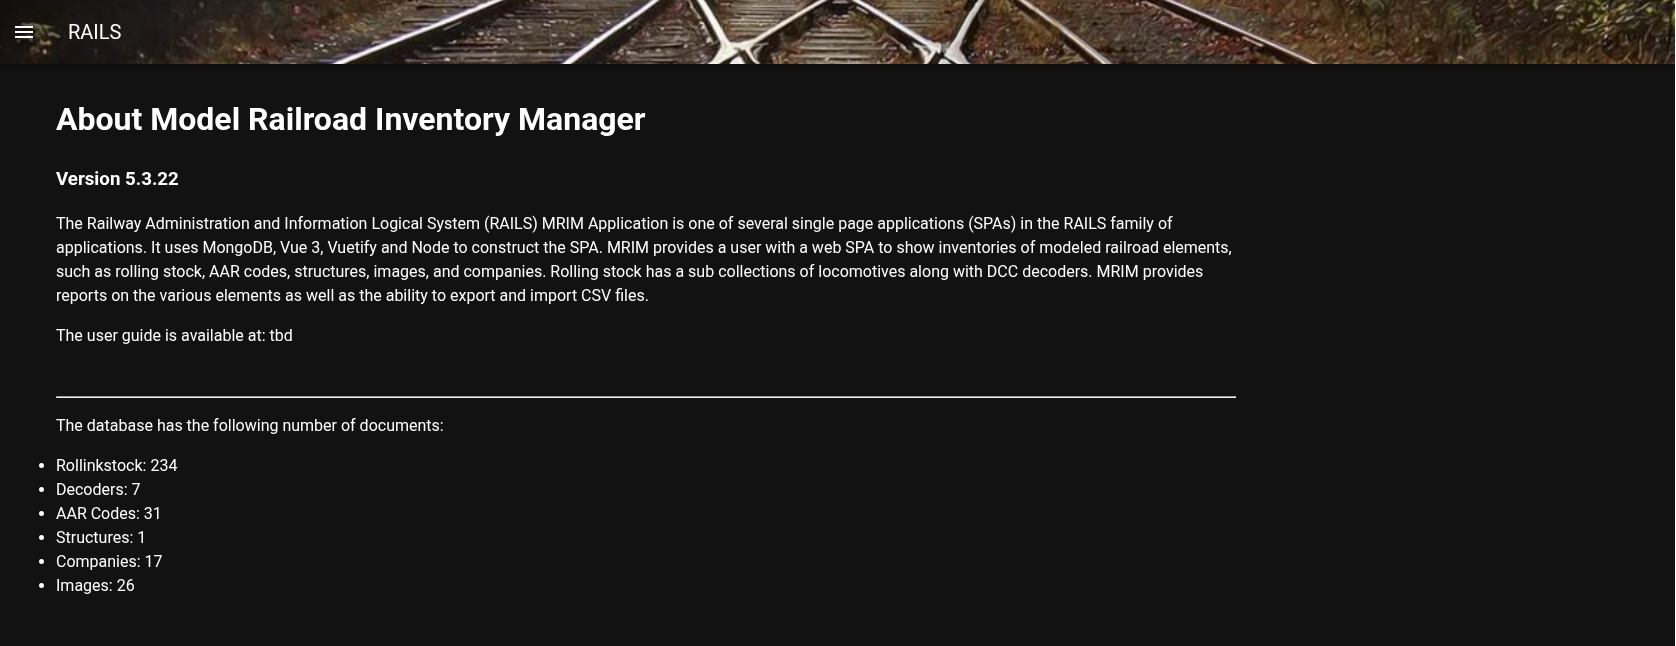
\includegraphics[scale=0.25]{./images/about.png}
    \caption{About Page}
    \label{fig:about1}
\end{figure}

The hamburger menu icon \hamburger, to the left of "RAILS" represents a hidden navigation menu that can be toggled open and closed. 
When the icon is clicked or tapped on the menu for navigation to different pages of this application is revealed. This menu  
contains the links: "Reader," "Admin," "Rollingstock," "AAR Codes," "About" (this page). 
Figure \ref{fig:about2} shows the "About" page with the navigation menu opened.

\begin{figure}[H]
    \centering
    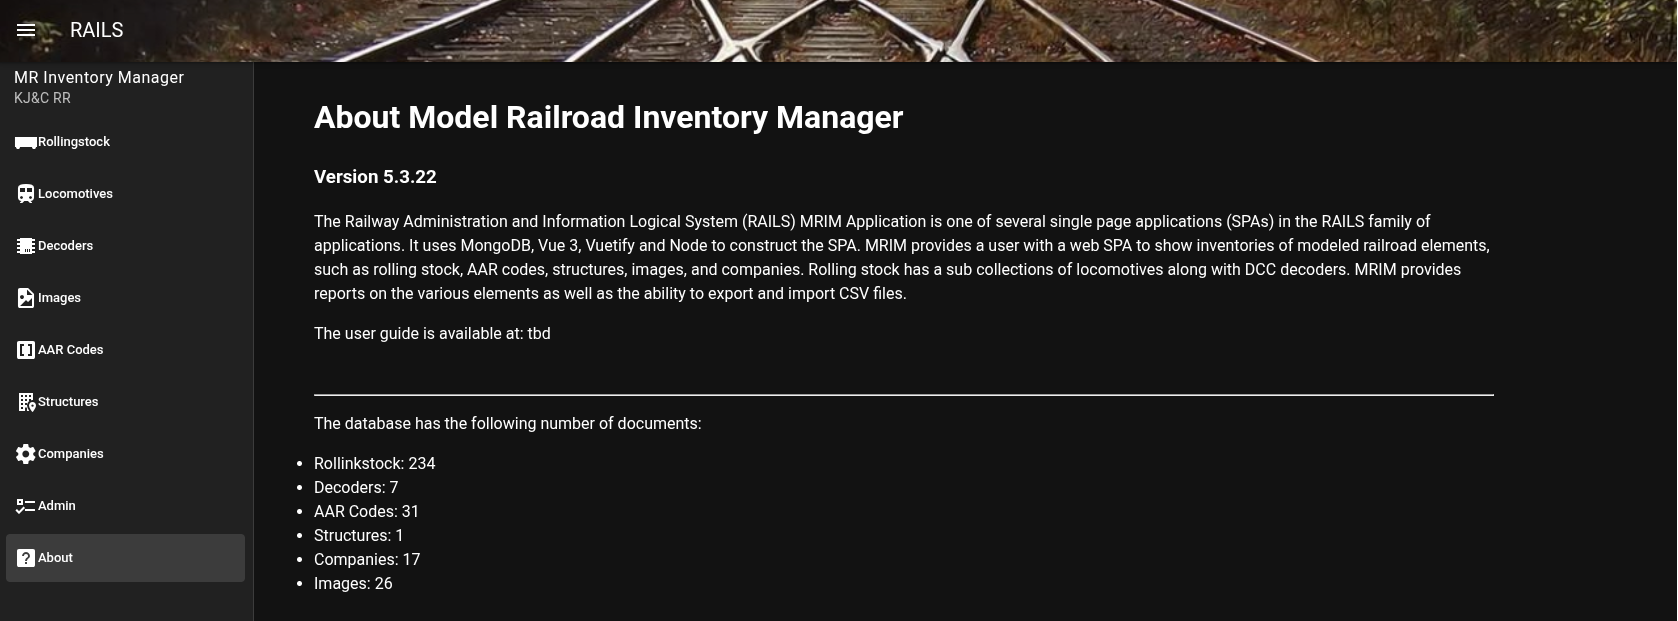
\includegraphics[scale=0.25]{./images/about-hamburger.png}
    \caption{Sidemenu}
    \label{fig:about2}
\end{figure}
